\section{Background} \label{background}
This section describes the background of this proposal and contains information that is available but might not be known by students and readers. 

\subsection{History of GUI testing}

% what is GUI testing?
% What role place GUI testing in the testing spectrum? (compared with unit / integration testing)
% First we had manually testing as old as the start of development -> Capture and Replay CR -> CR becomes automated -> scripted (monkey testing).

\subsection{What is TESTAR?}
TESTAR - or TEST* - is an automated software testing tool for the GUI level \cite{testar-about}. TESTAR started within the context of the \acrfull{fittest} project. TESTAR is open-source, the source code is published on GitHub \footnote{ \url{https://github.com/TESTARtool/TESTAR\_dev}}. A screenshot of the TESTAR tool is displayed in figure \ref{fig:testar}.

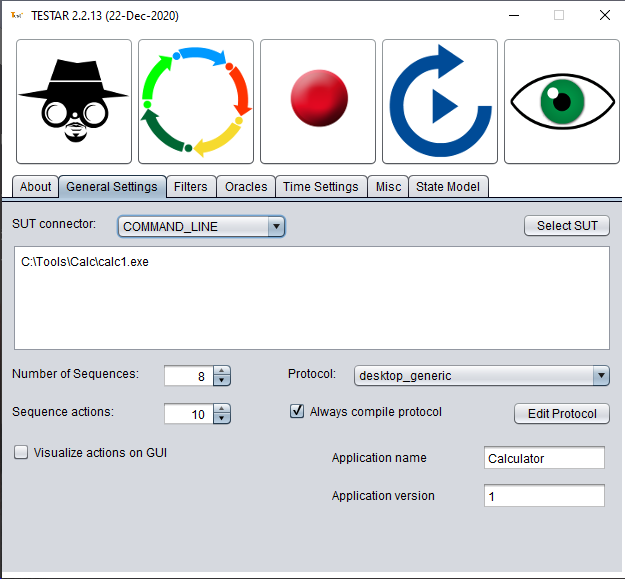
\includegraphics[scale=0.5]{pics/testar.png}
\captionof{figure}{Screenshot of the TESTAR tool}\label{fig:testar}

TESTAR has several \emph{execution modes} in which it interacts with the SUT \cite{testar-manual}. From left to right, in figure \ref{fig:testar}, those are Spy, Generate, Record, Replay and View mode. 

The \emph{Spy} mode allows the user to inspect a SUT and "see" how TESTAR is interpreting the widgets on the screen. Figure \ref{fig:calc-spy} shows the Windows calculator in spy mode. Dots on the GUI indicates actions with which TESTAR can interact. Within TESTAR, it is possible to filter actions. TESTAR will then not execute these actions. The actions are given a silver dot colour. A list with properties about the widget is shown when hovering, as well as a unique identifier of the current \emph{state}, more information about the state and the unique identifier can be found at section \ref{gui-state}.\par

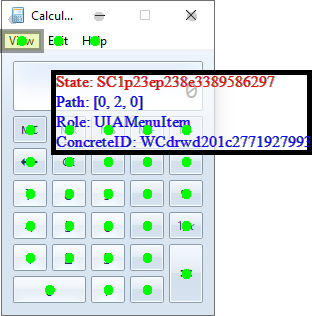
\includegraphics{pics/calc-state.png}
\captionof{figure}{Screenshot of the Calculator with TESTAR Spy}\label{fig:calc-spy}

In the \emph{Generate} mode will TESTAR will start testing the specified system. Section \ref{testar-testauto} for more detail about TESTAR test automation. \par

The \emph{Record} mode allows a tester to record a test sequence manually. In the \emph{Replay} mode, existing test execution can be re-executed and lastly, in the \emph{Review} mode allows existing test executions to be viewed. \par

\subsubsection{TESTAR automation} \label{testar-testauto}
    
TESTAR works without any test scripts but is uses GUI Ripper and Monkey testing techniques. \emph{GUI Ripping}, first introduced by Memon et al. \cite{gui-ripping}, is a process to obtain the GUI's structure and execution behaviour automatically. \emph{Monkey testing} is a process in which decisions are randomly chosen. 

    % -> tool to (smart) monkey test GU -> 
    % maybe copy figure 1 in here as a reference. 
    % The state is being checked with a test oracle (next section).

\subsection{How is the SUT tested}
When software is tested, a method is needed to check the correct behaviour of the SUT. The method of checking is formally known as a \emph{test oracle} \cite{testOracles}. An example of a test oracle widely used by developers is the code \emph{assertions}, which is a Boolean assertion. Developers can create assertions in software to check its behaviour during runtime \cite{barr2014oracle}. Assertions can also be used in unit tests as displayed by listing \ref{code:assert}. 

%% do not indent code since it indents its extra in the LaTeX output
\begin{lstlisting}[language=Java, caption=Assertion, label=code:assert]
@Test
public void testAdd(){
    Calculator sut = new Calculator();

    int expected = 3;
    int actual = sut.Add(1,2);

    Assert.assertEquals(expected, actual);
}
\end{lstlisting}

\subsubsection{Online and Offline Test oracles}
Test oracle comes in two variants, \emph{online} or \emph{on-the-fly} test oracle and \emph{offline} test oracles \cite{VosAho2021}. With online test oracles, the state under test is being asserted for any anomalies during test execution. For example,  an online test oracle inspects the URL to check for any information being exposed in the query string. Offline test oracles will look into stored data - like logs - to find anomalies after test execution. For example, offline test oracles can inspect all the visited URL's to check for any exposed information in the query strings.

Each variant come with their strengths and weaknesses. The online test oracle takes up compute time because it inspects the state during test execution. This inspecting of state slows down the test execution and may become an issue with time-critical SUT's. On the other hand, some issues - like the SUT become unresponsive - can only be checked during test execution. An offline test oracle is inspecting data that is gathered when test execution has finished. Especially with larger data sets, this can become helpful. Inspecting the data may run in parallel, which can speed up the test oracle. Additionally, when developers create new offline test oracles, they can inspect the recorded data instead of executing a new test run. \cite{de2019offline}

Besides the online and offline test oracle variants, test oracles can also be places under four categories. Barr et al. conducted a survey and classify test oracles into four categories. In Section \ref{to:four-cat} the four categories are explained. 

\subsubsection{Four categories} \label{to:four-cat}

% TESTAR has some built-in oracles. but can also be created.

\subsection{How is data retrieved}

Section \ref{testar-testauto} discussed how TESTAR is using GUI ripping to obtain the GUI's structure. A GUI exists out of a non-empty set of UI components, known as \emph{widgets}. Examples of widgets is a Window or a button; more examples can be found in table \ref{tables:widgets} \cite{VosAho2021}. The widgets are structured hierarchy in a \emph{widget tree}. Each node in the tree is a widget with its related properties, such as the title, position, and role.

\begin{tabularx}{\textwidth}{ 
  | >{\raggedright\arraybackslash}X 
  | >{\raggedright\arraybackslash}X 
  | >{\raggedright\arraybackslash}X | }
    \hline
    Windows & Menus & Controls \\
    \hline
    \hline
    main windows & menu bars & buttons \\
    child windows & dropdown menus & textbox \\
    popup windows & context-aware menus & links \\
    && radio buttons \\
    && checkboxes\\
    && dropdown select boxes\\
    && sliders\\
    && tabs\\
    && scrollbars \\
    \hline
\end{tabularx}
\captionof{table}{Example of GUI widgets \cite{VosAho2021}}\label{tables:widgets}

 The widgets are structured hierarchy in a \emph{widget tree}. Each node is a widget with its corresponding properties inside the tree, such as the title, position, and role. In figure \ref{fig:widget-tree} a compact widget tree is shown for the calculator. 

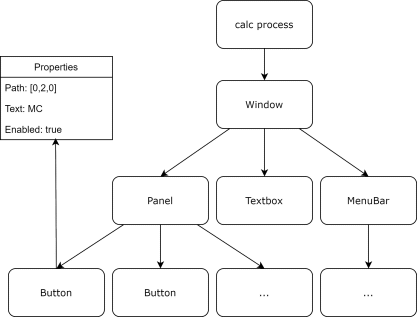
\includegraphics{pics/calc-tree.png}
\captionof{figure}{A compact version of a widget tree for the calculator.}\label{fig:widget-tree}

%% Windows Automation API.
%% JavaAccessBridge
%% Selenium Chromedriver
%\subsubsection{Windows Automation API}
%\subsubsection{JavaAccessBridge}
%\subsubsection{Selenium Chromedriver}

%background questions. what is now and what do we already have
%- what is a model? -> Background
    % What is a widget -> obtaining state with widgets -> generate action set -> selection action.

\subsubsection{GUI State} \label{gui-state}
%state is an application in state -> 

\subsection{How is data persisted}

TESTAR is using a database to store and retrieve state model data. Gier and Kager investigated which data storing solution would be beneficial to TESTAR \cite{GierKager}. The data solution must comply with six requirements. Generally speaking, the requirements were as follows: an open-source graph database with a straightforward query mechanic. The conclusion was that OrientDB was the best solution that met all the requirements.

OrientDB is a Multi-Model NoSQL \acrfull{dbms} that combines four models \cite{orientDbModeling}:

\begin{itemize}
    \item \hyperlink{db:key-value}{Key/Value}
    \item \hyperlink{db:document}{Document}
    \item \hyperlink{db:graph}{Graph}
    \item \hyperlink{db:object}{Object}
\end{itemize}

A \hypertarget{db:key-value}{\emph{Key/Value}} is the simplest model and allows storing information (value) that is accessible with a key. Key/Values can be group into \textit{buckets} however, OrientDB support richer models in the form of document and graph elements.

A \hypertarget{db:document}{\emph{document}} is a schema-less set of key/value pairs. The \emph{key} allows access to the corresponding value. OrientDB allows the developer to store documents into \emph{clusters}. Relations between document are either embedded into other document or \emph{linked} to each other. Someone familiar with relational databases can view a cluster as tables, a document as the row and the key/value pairs are columns.

The \hypertarget{db:graph}{\emph{graph}} is a model consisting of \emph{Vertices} and \emph{Edges}. Vertices are the nodes in the graph, and the edge is the link between those nodes. In TESTAR terminology, a vertex represents state, and the edge is an 'action' from one state to the next. A Vertex consists of three elements: a unique identifier, a set with incoming Edges and outgoing Edges. An edge consists of four elements: a unique identifier, an incoming vertex (\emph{head}), an outgoing vertex (\emph{tail}) and a label that describes the relationship between the head and tail vertex.\par

The last model is the \hypertarget{db:object}{\emph{object}}, which supports inheritance like in the Object-Oriented programming paradigm.\par

Despite being a NoSQL database, OrientDB does support SQL as a query language \cite{sql-lang} albeit that it does not support all SQL statements. The majority of developers have experience with SQL \cite{sql-stats} as a result, new developers and students can start querying the TESTAR data and start expanding its features.\par

In addition to TESTAR, other application can query the state model data in the OrientDB database as well. For example, developers en students can create external tools for a single purpose, like a state model difference application. When building external tools, the TESTAR application can be kept small and focus upon one objective: testing GUI applications. 